\documentclass[conference]{IEEEtran}
\IEEEoverridecommandlockouts
\usepackage{cite}
\usepackage{amsmath}
\usepackage{graphicx}
\usepackage{booktabs}
\usepackage{textcomp}
\usepackage[hidelinks]{hyperref}
\newcommand{\NOrders}{10,977}
\newcommand{\NTrain}{8,421}
\newcommand{\NTest}{2,106}
\newcommand{\NSeeds}{5}
\newcommand{\MaeGB}{1.47}
\newcommand{\MaeOwn}{1.58}
\newcommand{\MaeEWMA}{1.45}
\newcommand{\MaeSeg}{2.42}
\newcommand{\GainOwn}{6.5}
\newcommand{\GainEWMA}{-1.5}
\newcommand{\WithinTwo}{75.2}
\newcommand{\Rmse}{2.03}
\newcommand{\CovGBThree}{92.8}
\newcommand{\CovGBThreeLead}{2.8}
\newcommand{\CovGBZero}{35.6}
\newcommand{\CovOwnThree}{95.3}
\newcommand{\TopFeature}{ewm\_int}
\newcommand{\TopFeatureShare}{80}
\newcommand{\TopTwoShare}{87}
\newcommand{\TableMae}{%
\begin{tabular}{lcccc}
\toprule
Model & $\sigma\times$0.5 & $\sigma\times$1 & $\sigma\times$2 & $\sigma\times$3 \\
\midrule
Segment mean & 2.14\,$\pm$\,0.06 & 2.42\,$\pm$\,0.08 & 3.10\,$\pm$\,0.10 & 3.75\,$\pm$\,0.20 \\
Own mean & 1.21\,$\pm$\,0.03 & 1.58\,$\pm$\,0.06 & 2.47\,$\pm$\,0.11 & 3.26\,$\pm$\,0.18 \\
Last gap & 0.94\,$\pm$\,0.03 & 1.67\,$\pm$\,0.13 & 3.13\,$\pm$\,0.13 & 4.24\,$\pm$\,0.29 \\
EWMA & 0.90\,$\pm$\,0.03 & 1.45\,$\pm$\,0.09 & 2.62\,$\pm$\,0.13 & 3.54\,$\pm$\,0.21 \\
Ridge & \textbf{0.88\,$\pm$\,0.03} & \textbf{1.38\,$\pm$\,0.07} & \textbf{2.41\,$\pm$\,0.11} & \textbf{3.23\,$\pm$\,0.17} \\
Random forest & 0.91\,$\pm$\,0.05 & 1.45\,$\pm$\,0.07 & 2.58\,$\pm$\,0.13 & 3.47\,$\pm$\,0.22 \\
Gradient boosting & 0.96\,$\pm$\,0.05 & 1.47\,$\pm$\,0.12 & 2.61\,$\pm$\,0.28 & 3.44\,$\pm$\,0.33 \\
\bottomrule
\end{tabular}}
\newcommand{\TableLead}{%
\begin{tabular}{ccccc}
\toprule
Lead & \multicolumn{2}{c}{Own mean} & \multicolumn{2}{c}{Gradient boosting} \\
(days) & Useful (\%) & Notice (d) & Useful (\%) & Notice (d) \\
\midrule
0 & 48.2 & 1.7 & 35.6 & 1.4 \\
1 & 70.1 & 2.0 & 62.4 & 1.6 \\
2 & 87.8 & 2.5 & 83.0 & 2.1 \\
3 & 95.3 & 3.3 & 92.8 & 2.8 \\
5 & 98.9 & 5.1 & 98.5 & 4.6 \\
7 & 99.7 & 7.1 & 99.7 & 6.5 \\
\bottomrule
\end{tabular}}
\newcommand{\TableSeg}{%
\begin{tabular}{lrrr}
\toprule
Segment & Gap & Own & GB \\
\midrule
Catering & 6.5 & 1.32 & 1.06 \\
Hotel & 7.4 & 1.54 & 1.23 \\
Canteen / Hostel & 8.9 & 1.53 & 1.87 \\
Restaurant & 11.7 & 1.47 & 1.50 \\
Bakery & 13.7 & 1.69 & 1.65 \\
Street Food & 17.7 & 2.17 & 2.17 \\
Industrial & 25.7 & 3.30 & 3.40 \\
\bottomrule
\end{tabular}}
 % numbers below are generated by experiments.py, not typed by hand

\begin{document}

\title{Predictive Restocking and Automated Booking for a Commercial Gas-Cylinder Distributor: A Synthetic-Data Study}

\author{\IEEEauthorblockN{Author Name}
\IEEEauthorblockA{\textit{Department / Organisation}\\
City, Country\\
author@example.com}}

\maketitle

\begin{abstract}
Small commercial gas-cylinder distributors serve restaurants, hotels, bakeries and caterers that must never run out of fuel, yet most dealers learn that a customer needs cylinders only when the customer calls. This paper describes a web platform that predicts each customer's next refill date from order history, emails a signed one-click booking link shortly before the predicted date, and gives the dealer a dashboard of revenue, margin and receivables. Because no real order history was available, the platform was developed and evaluated on a synthetic population of 150 customers in seven business segments. On a chronological hold-out, a gradient-boosting predictor reaches a mean absolute error of \MaeGB{} days, \GainOwn\% lower than each customer's own mean gap (\MaeOwn{} days) but no better than a recency-weighted average (\MaeEWMA{} days), and ridge regression is lowest at every noise level tested. We report these results as they are: on this generator, simple models are sufficient, and the study says nothing yet about real customers. The code, generator and experiment scripts accompany the paper.
\end{abstract}

\begin{IEEEkeywords}
demand forecasting, replenishment prediction, gradient boosting, synthetic data, small business software, web application
\end{IEEEkeywords}

\section{Introduction}
A commercial gas dealer sells cylinders to a modest number of repeat customers. Each customer consumes gas at a fairly steady rate, so the interval between refills is regular but not constant: it varies with trade, season, and demand. A customer who runs out stops cooking, and a dealer who cannot anticipate demand either over-stocks cylinders or delivers late. A reminder sent a few days before the customer runs out, with an easy way to book, serves both sides.

We built a complete system around that idea: customer and dealer portals, a restock predictor, a reminder scheduler, and a finance dashboard. The research question we can honestly address with the data at hand is narrow: \emph{given only a customer's past delivery dates and quantities, how accurately can the next delivery date be predicted, and is a learned model worth its complexity over simple rules?} Our contributions are:
\begin{itemize}
\item an open, end-to-end architecture for prediction-driven reminders and booking (Section~\ref{sec:arch});
\item a parameterised synthetic-order generator with per-customer rhythm, seasonality, trend and noise (Section~\ref{sec:data});
\item a multi-seed comparison of seven predictors, and an analysis of how the reminder lead time trades timeliness against notice (Section~\ref{sec:results}).
\end{itemize}
The central empirical finding is negative for the more complex models, and the main limitation is that all data are synthetic (Section~\ref{sec:limits}).

\section{Background and Related Work}
Replenishment timing is related to customer-base analysis, where models such as Pareto/NBD \cite{schmittlein1987} and its simpler successor BG/NBD \cite{fader2005} estimate purchase rates and ``alive'' probabilities from transaction histories. Those models target non-contractual customers who may churn; here, customers are contractual-like repeat buyers and the question is the \emph{timing} of the next purchase rather than whether it will occur. Intermittent-demand methods such as Croston's \cite{croston1972} address irregular, sparse demand for stock control, whereas our interval target is dense and regular. Exponential smoothing \cite{brown1959} is the classical way to weight recent observations; we use it both as a baseline and as an input feature.

On the learning side we compare gradient boosting \cite{friedman2001}, random forests \cite{breiman2001}, and ridge regression \cite{hoerl1970}, all as implemented in scikit-learn \cite{pedregosa2011}. For evaluation we use mean absolute error, which is scale-dependent but directly interpretable in days \cite{hyndman2006}, and a chronological split, because random splits of temporally ordered data can overstate accuracy \cite{bergmeir2012}.

\section{System Architecture}\label{sec:arch}
Fig.~\ref{fig:arch} shows the four layers. The application is a single Python service (FastAPI) with server-rendered pages and a SQLite database, chosen so that a one-person business can run it on a Windows laptop by opening one file.

\begin{figure*}[t]
\centering
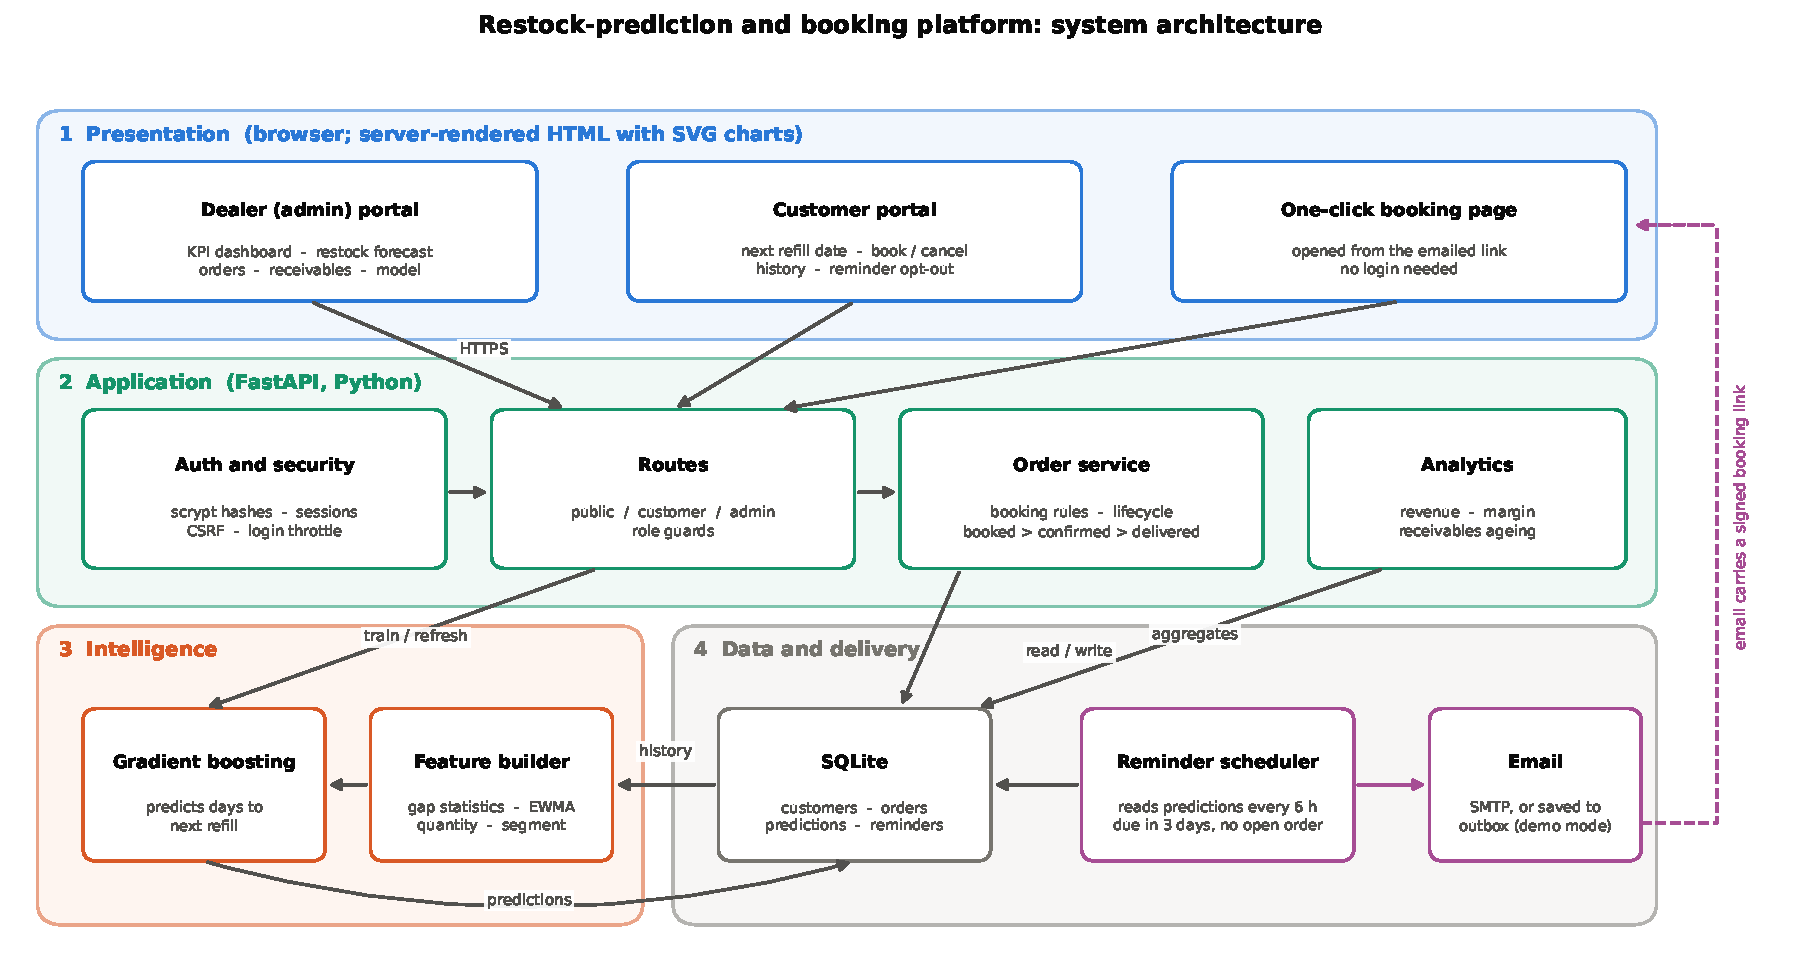
\includegraphics[width=0.92\textwidth]{figures/fig_architecture.pdf}
\caption{System architecture. Solid arrows are requests and data flow; the dashed purple path is the reminder email, which carries a signed booking link back to the one-click booking page.}
\label{fig:arch}
\end{figure*}

\subsection{Presentation and application layers}
Three browser interfaces share one service: a dealer portal (dashboard, restock forecast, orders, receivables, e-mail log, model page), a customer portal (next expected refill, booking, history, outstanding balance, reminder opt-out) and a booking page opened from an email. The dashboard reports revenue, gross profit and margin, cylinders delivered, mean cylinders per order and per customer per month, revenue per cylinder, receivables ageing from each customer's credit terms, and collections.

Passwords are stored with scrypt ($N{=}2^{14}$, $r{=}8$, $p{=}1$) \cite{percival2009}; sessions are signed cookies regenerated at login; every state-changing form carries a per-session CSRF token; and logins are throttled to six failures per ten minutes per address and client. Customers may only act on their own orders, and dealer pages are reachable only with the dealer role. Login is by email and password only, with no second factor; a deployment on the public internet should add one.

\subsection{Order lifecycle and reminders}
An order moves from \emph{booked} to \emph{confirmed} to \emph{delivered} (or \emph{cancelled}). A customer may hold at most one open booking. Marking an order delivered immediately recomputes that customer's prediction, so the forecast always reflects the latest delivery.

A scheduler runs every six hours. For each customer whose predicted restock date is within three days, who has no open booking and has not opted out, it sends one email per refill cycle (keyed by customer and last delivery date). The email contains a link whose token is an HMAC-signed, time-limited (14-day) payload holding the customer, suggested product and quantity; tampering or expiry yields an error page. The customer can change size, quantity and date before confirming. Without an SMTP server, messages are written to a local outbox, so the flow can be exercised offline.

\section{Synthetic Data}\label{sec:data}
No real order history was available, so we generate it. The generator is deliberately transparent so that the structure the models can learn is known exactly.

\textbf{Population.} Customers belong to seven segments (restaurant, hotel, bakery, catering, canteen/hostel, street food, industrial), each with a baseline refill interval from 7 to 26 days, a typical quantity, a usual cylinder size and credit terms. Each customer's interval is the segment baseline times a personal factor drawn uniformly from $[0.7, 1.4]$, so two restaurants differ systematically.

\textbf{Dynamics.} For each customer we simulate 730 days of deliveries. The gap before the next order is the personal interval divided by a rate that combines (i) segment seasonality (catering and hotels consume 35\% faster from October to February; bakeries 30\% faster in December and January; canteens 40\% slower in May and June), and (ii) a linear trend in consumption drawn from $[-15\%, +25\%]$ over the period, then multiplied by Gaussian noise with a relative standard deviation drawn from $[0.05, 0.22]$ per customer. Deliveries skip Sundays, quantities vary by about 20\%, and payment delay depends on credit terms. A global \emph{noise scale} $\sigma$ multiplies the noise term; $\sigma{=}1$ is the default used by the application and $\sigma\in\{0.5,1,2,3\}$ is used in the experiments. The default population contains \NOrders{} delivered orders.

\textbf{Prices.} Selling prices are INR 2{,}900 (19\,kg) and INR 4{,}500 (33\,kg). Cost prices were not available and are set 10\% below selling price as a placeholder, so margin figures in the dashboard are illustrative.

\section{Prediction Method}\label{sec:method}
\textbf{Task.} For a customer with deliveries $d_1<\dots<d_k$ ($k\ge 3$), predict the next gap $g_{k+1}=d_{k+1}-d_k$ in days; the restock date is $d_k+\hat g_{k+1}$.

\textbf{Features.} Twenty features are computed from history up to $d_k$ only: the last three gaps; their mean, standard deviation and exponentially weighted mean (EWMA, $\alpha{=}0.5$); last and mean quantity; number of orders and tenure; weekday and month of the last delivery; the segment's baseline interval; and a one-hot segment indicator.

\textbf{Models.} Four rule-based baselines predict the segment baseline, the customer's mean gap, the last gap, or the EWMA. Three learned models use all features: ridge regression (standardised, $\alpha{=}1$), a random forest (200 trees, minimum leaf size 5), and gradient boosting (300 trees, depth 3, learning rate 0.05, subsample 0.8, absolute-error loss), which is the model deployed in the application. Hyper-parameters were fixed in advance and not tuned.

\textbf{Protocol.} All examples (one per delivery with at least three predecessors) are ordered by the date of the last known delivery. The earlier 80\% train the models and the later 20\% test them, so no model sees the future. The first replicate has \NTrain{} training and \NTest{} test examples. We repeat the whole pipeline, including data generation, for \NSeeds{} seeds and report mean $\pm$ sample standard deviation across seeds.

\section{Results}\label{sec:results}

\subsection{Accuracy}
Table~\ref{tab:mae} gives test MAE. At the default noise ($\sigma{=}1$), gradient boosting reaches \MaeGB{} days, \GainOwn\% better than the customer's own mean gap (\MaeOwn{} days) and far better than the segment baseline (\MaeSeg{} days), but \emph{not} better than the EWMA baseline (\MaeEWMA{} days; boosting is within 1.5\% of it, inside the seed-to-seed spread). Ridge regression has the lowest MAE at every noise level (1.38 days at $\sigma{=}1$), and the random forest (1.45) matches EWMA. About \WithinTwo\% of boosting predictions fall within two days of the truth (RMSE \Rmse{} days).

\begin{table*}[t]
\caption{Test MAE in days (mean $\pm$ s.d. over \NSeeds{} seeds) by model and noise scale. Lowest per column in bold.}
\label{tab:mae}
\centering\small
\TableMae
\end{table*}

Fig.~\ref{fig:noise} shows that all methods degrade as behaviour becomes more irregular, and that the gap between learned models and the own-mean baseline narrows: at $\sigma{=}3$ ridge is the only model that is better than own-mean at all, by about 1\%, while boosting is worse (3.44 vs.\ 3.26 days). Gradient boosting also has the largest seed-to-seed variance at higher noise ($\pm$0.28 at $\sigma{=}2$).

\begin{figure}[t]
\centering
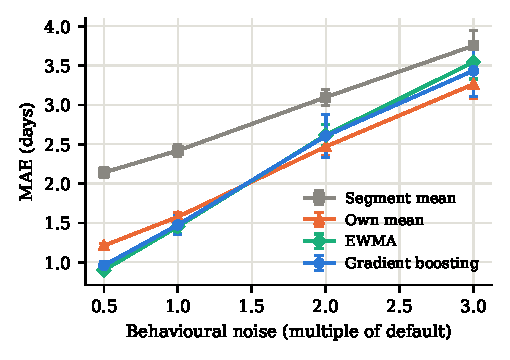
\includegraphics[width=\columnwidth]{figures/fig_mae_noise.pdf}
\caption{Test MAE versus behavioural noise (error bars: s.d. over \NSeeds{} seeds).}
\label{fig:noise}
\end{figure}

\subsection{What the model uses}
The boosted model's impurity-based importance is dominated by the recency-weighted gap: \texttt{\TopFeature} carries \TopFeatureShare\% and the top two features (EWMA and mean gap) \TopTwoShare\%. This agrees with the baseline results: most of the predictable signal is each customer's recent rhythm. Month of year, although it drives seasonality in the generator, carries only about 3\%. Impurity importance is known to be biased and we did not test this further.

\subsection{By segment}
Table~\ref{tab:seg} breaks the default-noise results down by segment. Boosting is clearly better than the own-mean rule for catering (1.06 vs.\ 1.32 days) and hotels (1.23 vs.\ 1.54), the segments with the strongest seasonality in the generator, is equal for street food, restaurants and bakeries, slightly worse for industrial customers (3.40 vs.\ 3.30, the segment with the fewest test examples), and clearly \emph{worse} for canteens and hostels (1.87 vs.\ 1.53). We did not investigate the latter. Absolute error grows with the length of the gap (3.4 days for industrial customers with a 26-day gap), but boosting's error relative to the mean gap is similar across segments (roughly 12--21\%).

\begin{table}[t]
\caption{Default-noise results by segment, ordered by mean gap. Gap = mean days between refills; Own and GB = test MAE in days of the own-mean rule and gradient boosting.}
\label{tab:seg}
\centering\small
\TableSeg
\end{table}

\subsection{Reminder lead time}
A reminder sent $L$ days before the predicted date is \emph{in time} if the customer has not yet reordered, i.e.\ the actual gap is at least $\hat g - L$. The \emph{notice} is the mean number of days between the reminder and the actual reorder, among in-time reminders. Table~\ref{tab:lead} and Fig.~\ref{fig:lead} show the trade-off, pooled over seeds at $\sigma{=}1$. With the deployed three-day lead, \CovGBThree\% of boosting reminders arrive in time with \CovGBThreeLead{} days of notice on average; the own-mean rule is in time more often (\CovOwnThree\%) with slightly more notice. Sending on the predicted date itself (lead 0) would be in time only \CovGBZero\% of the time.

The boosting model's errors are biased: customers reorder on average about 0.5 days \emph{earlier} than predicted (mean of actual minus predicted $-0.5\pm0.2$ days). This is consistent with the generator's positive average consumption trend, which shortens later gaps, and with an absolute-error loss that targets the median, but we did not isolate the cause. Because timeliness is asymmetric (a late reminder is worse than an early one), a practical deployment should choose the lead from a target in-time rate, for example five days for roughly 98\% here, rather than minimise MAE alone.

\begin{table}[t]
\caption{Reminder lead time at default noise: share of reminders sent before the customer reorders, and mean days of notice.}
\label{tab:lead}
\centering\footnotesize
\TableLead
\end{table}

\begin{figure}[t]
\centering
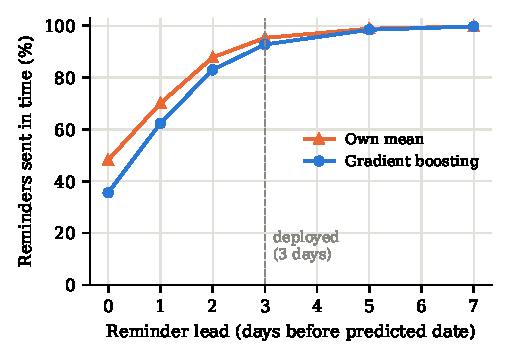
\includegraphics[width=\columnwidth]{figures/fig_lead.pdf}
\caption{Share of reminders sent in time versus lead; the deployed lead is three days.}
\label{fig:lead}
\end{figure}

\begin{figure}[t]
\centering
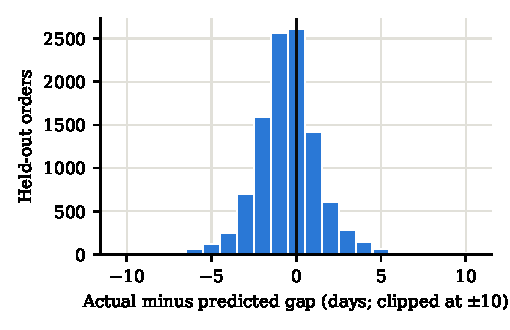
\includegraphics[width=\columnwidth]{figures/fig_error_hist.pdf}
\caption{Distribution of actual minus predicted gap for gradient boosting on held-out orders (pooled over seeds, clipped at $\pm$10 days).}
\label{fig:hist}
\end{figure}

\section{Discussion and Limitations}\label{sec:limits}
\textbf{All data are synthetic.} The results measure how well each method recovers the structure we put into the generator. They cannot show how accurate the predictor would be for real customers, whose consumption is affected by stock-outs, price changes, holidays, multiple sites, delivery bundling and dealer-side delays that the generator omits. The ranking of models could change on real data; in particular, tree ensembles often gain over linear models when relationships are non-linear, and our generator is close to multiplicative-linear in the gaps. The absolute errors reported here should not be quoted as expected real-world performance.

\textbf{Simple models are sufficient here.} Because EWMA and ridge match or beat the boosted model, a dealer with limited data loses little by using a recency-weighted average, which is also easier to explain to customers. The learned model's advantages are confined to the seasonal segments. We therefore recommend retraining and re-comparing on a few months of real orders before trusting any of the models, and the application exposes retraining and the hold-out metrics for that purpose.

\textbf{Other limitations.} We use a single chronological split per replicate and fixed hyper-parameters, no confidence intervals beyond seed variance, and we did not evaluate the prediction window shown to the dealer. The platform's practical value (booking conversion, reduction in stock-outs, dealer time saved) was not measured; no users have yet used the system. Cost prices are placeholders, and authentication has no second factor.

\section{Conclusion}
We presented an open platform that turns order history into timely, bookable reminders for a commercial gas dealer, together with a synthetic-data benchmark and an honest comparison of predictors. On synthetic data, gradient boosting improves on each customer's average gap by \GainOwn\% but is matched by a recency-weighted average and bettered slightly by ridge regression, and the choice of reminder lead time matters more for timeliness than the choice of model. The next step is a pilot with real order history to test whether these conclusions hold.

\section*{Reproducibility}
\raggedright All tables and figures are produced by \texttt{experiments.py} and \texttt{make\_architecture.py} in the \texttt{research} folder of the project repository. Tables and headline numbers are read from the generated \texttt{results.tex}; the remaining values in Section~\ref{sec:results} were copied by hand from the generated tables and from \texttt{results.json}.

\begin{thebibliography}{00}
\bibitem{schmittlein1987} D. C. Schmittlein, D. G. Morrison, and R. Colombo, ``Counting your customers: Who are they and what will they do next?'' \emph{Management Science}, vol. 33, no. 1, pp. 1--24, 1987.
\bibitem{fader2005} P. S. Fader, B. G. S. Hardie, and K. L. Lee, ``Counting your customers the easy way: An alternative to the Pareto/NBD model,'' \emph{Marketing Science}, vol. 24, no. 2, pp. 275--284, 2005.
\bibitem{croston1972} J. D. Croston, ``Forecasting and stock control for intermittent demands,'' \emph{Operational Research Quarterly}, vol. 23, no. 3, pp. 289--303, 1972.
\bibitem{brown1959} R. G. Brown, \emph{Statistical Forecasting for Inventory Control}. New York: McGraw-Hill, 1959.
\bibitem{friedman2001} J. H. Friedman, ``Greedy function approximation: A gradient boosting machine,'' \emph{Annals of Statistics}, vol. 29, no. 5, pp. 1189--1232, 2001.
\bibitem{breiman2001} L. Breiman, ``Random forests,'' \emph{Machine Learning}, vol. 45, no. 1, pp. 5--32, 2001.
\bibitem{hoerl1970} A. E. Hoerl and R. W. Kennard, ``Ridge regression: Biased estimation for nonorthogonal problems,'' \emph{Technometrics}, vol. 12, no. 1, pp. 55--67, 1970.
\bibitem{pedregosa2011} F. Pedregosa \emph{et al.}, ``Scikit-learn: Machine learning in Python,'' \emph{Journal of Machine Learning Research}, vol. 12, pp. 2825--2830, 2011.
\bibitem{hyndman2006} R. J. Hyndman and A. B. Koehler, ``Another look at measures of forecast accuracy,'' \emph{International Journal of Forecasting}, vol. 22, no. 4, pp. 679--688, 2006.
\bibitem{bergmeir2012} C. Bergmeir and J. M. Ben{\'\i}tez, ``On the use of cross-validation for time series predictor evaluation,'' \emph{Information Sciences}, vol. 191, pp. 192--213, 2012.
\bibitem{percival2009} C. Percival, ``Stronger key derivation via sequential memory-hard functions,'' in \emph{BSDCan}, 2009.
\end{thebibliography}

\end{document}
